%% Copyright 1998 Pepe Kubon
%%
%% `two.tex' --- 2nd chapter for thes-full.tex, thes-short-tex from
%%               the `csthesis' bundle
%%
%% You are allowed to distribute this file together with all files
%% mentioned in READ.ME.
%%
%% You are not allowed to modify its contents.
%%

%%%%%%%%%%%%%%%%%%%%%%%%%%%%%%%%%%%%%%%%%%%%%%%%%
%
%     Chapter 4  
%
%%%%%%%%%%%%%%%%%%%%%%%%%%%%%%%%%%%%%%%%%%%%%%%%

\chapter{A Pruning-based Method On Graph}
\label{ch:graph}

In this section, we will introduce the algorithms to compute the skyline subspace queries. One way to solve this problem is to compute the label distance vectors of all the vertices first and enumerate all the subspaces to check whether the query vertex is a subspace skyline in those subspaces. This method could be very time consuming. In order to make the algorithm more efficient, we manage to avoid some unnecessary computations by applying some pruning techniques in our method.

\section{BFS Label Collecting}
\label{sec:bfs-collect}
We collect the d-hop labels by Breadth-First-Search and get the label vector. The idea is that we start with our query vertex and traverse the graph in the Breadth First order. If we visit a vertex with a new label that we have not visited before, we update the entry of that label in \emph{label distance vector} to the distance from query vertex. The Breadth First Search process will end if all reachable vertices in $d$ hops has been visited. And we will get the $label distance vector$ of the query vertex when the BFS label collecting ends.

\begin{algorithm}[H]
  \caption{Label Collecting}\label{algo:blah}
  \begin{algorithmic}[1]
  \show\LOOP
    \REQUIRE A graph $G=(V,E)$, a list of label sets $F=\left\{L_v | v \in V\right\}$, the label sets of all vertices, a query vertex $q$, the number of hops $d$;
    \ENSURE The label distance vector $LV_q$ of the query vertex $q$;
    \STATE push $\left(q, 0\right)$ to $Q$
    \WHILE {$Q$ is not empty}
        \STATE $\left( v, dis\right)$ = de-queue $Q$
        \IF{$dis=d$}
            \STATE continue
        \ENDIF
        \FORALL {not visited neighbour $u$ of $v$}
            \STATE push $\left(u, dis+1\right)$ to $Q$
            \FORALL {label $l$ in $L_u$}
                \IF {($l$, $\ast$) not in $LV_q$}
                    \STATE add ($l$, $dis+1$) to $LV_q$
                \ENDIF
            \ENDFOR
        \ENDFOR
    \ENDWHILE
  \end{algorithmic}
\end{algorithm}

\section{Dominating Candidates Set}
\label{sec:bfs-collect}

By collecting the label in $d$ hops from the query vertex, we build the label distance vector of our query vertex. To avoid computing the label distance vectors of all other vertices to find the skyline subspaces, we define a concept of dominating candidates set to compute the skyline subspaces.

\begin{definition}[Dominating Candidates Set]
Given a subspace $\mathcal{B}$, the dominating candidates set of that subspace is the set of vertices that dominate the query vertex $q$ or equal to query vertex $q$ in subspace $\mathcal{B}$, denoted by $\mathit{CAND}_\mathcal{B}$.
\end{definition}

Property~\ref{ppt:empty_cand}, shows that we can determine whether a subspace $\mathcal{B}$ is a \emph{skyline subspace} by checking the elements the \emph{dominating candidates set} of the subspace $\mathcal{B}$.

\begin{property}
\label{ppt:empty_cand}
If $\mathit{CAND}_\mathcal{B} = \emptyset$ or every vertex in $\mathit{CAND}_\mathcal{B}$ is equal to the query vertex $q$ in subspace $\mathcal{B}$, then $q$ is a skyline in subspace $\mathcal{B}$.
\end{property}

\begin{proof}
If $\mathit{CAND}_\mathcal{B} = \emptyset$ or every vertex in $\mathit{CAND}_\mathcal{B}$ is equal to the query vertex $q$ in subspace $\mathcal{B}$, then there is no vertex dominates the query vertex $q$ in $\mathit{CAND}_\mathcal{B}$.
$\mathit{CAND}_\mathcal{B}$ contains all the vertices that are not dominated by $q$. If all the vertices in $\mathit{CAND}_\mathcal{B}$ do not dominate $q$ in $\mathcal{B}$ then $q$ must be a skyline in subspace $\mathcal{B}$.
\end{proof}

\subsection{Dominating Candidates Set of $1$-dimensional subspace}

We will introduce an algorithm to compute the \emph{dominating candidates set} of $1$-dimensional subspace. We will also introduce the concepts of \emph{Strictly Dominating Subspace} and \emph{Equivalence Subspace} which help us prune the unnecessary dominating candidates.

\begin{definition}[Strictly Dominate]
In a label graph, we say that label distance vector $LV_v=\left\{(l_i, dist_i)\right\}$ dominates label vector $LV_u=\left\{(l_i, dist_i^\prime)\right\}$, if and only if for all i, $dist_i < dist_i^\prime$.
\end{definition}

\begin{definition}[Strictly Dominating Subspace]
Strictly dominating subspace $\mathcal{B}$ is the maximal subspace such that given a vertex $u$, $u_\mathcal{B}$ strictly dominates query vertex $q_\mathcal{B}$ on subspace $\mathcal{B}$.
\end{definition}

\begin{definition}[Equivalence Subspace]
Equivalence subspace $\mathcal{B}$ is the maximal subspace such that given a vertex $u$, if $u_\mathcal{B}$ equals to the query vertex $q_\mathcal{B}$ in subspace $\mathcal{B}$.
\end{definition}

In this algorithm, we start from the vertices with labels and update the label distance vector of those vertices. In the next step, we push all the neighbours of those vertices into the queue and update their label distance vectors and keep going. 
\begin{algorithm}[h]
  \caption{Dominating Candidates Set On $1$-Dimensional Subspace}\label{algo:blah}
  \begin{algorithmic}[1]
  \show\LOOP
    \REQUIRE A graph $G=(V,E)$ and the label vector $LV_q$ of the query vertex $q$;
    \ENSURE Dominating Candidates Set $\mathit{CAND}$ in all one dimension subspace in $LV_q$, $\mathit{EQS}$ and $\mathit{SDS}$;
    \FORALL {vertex $v$ contains label $l$}
        \FORALL {$\left(l, dist\right)$ in $LV_q$}
            \STATE push $\left(v, 0\right)$ to $Q$
        \ENDFOR
    \ENDFOR
    \WHILE {$Q \not= \emptyset$}
        \FORALL {$\left(l, dist\right)$ in $LV_q$}
            \STATE $\left(v, dist_{v,l}\right)$ = de-queue $Q$
            
            \IF{$dist_{v,l} = dist$}
                \STATE add $\left(u, equal\right)$ to $\mathit{CAND}_l$
                \STATE add $l$ to $\mathit{EQS}_u$
                \STATE continue
            \ENDIF
            \STATE add $\left(u, dom\right)$ to $\mathit{CAND}_l$
            \STATE add $l$ to $\mathit{SDS}_u$
            \FORALL {not visited neighbour $u$ of $v$}
                \STATE push $\left(u, dist_{v,l}+1\right)$ to $Q$
            \ENDFOR
        \ENDFOR
    \ENDWHILE
  \end{algorithmic}
\end{algorithm}

\subsection{Running Example of Computing Dominating Candidates Set}

In this subsection, we will give an example of how the algorithm of finding \emph{dominating candidates set on $1$-dimensional subspace} works. We will also show how the \emph{strictly dominating subspace} and the \emph{equivalence subspace} of each vertex is built.

\begin{figure}[H]
    \centering
    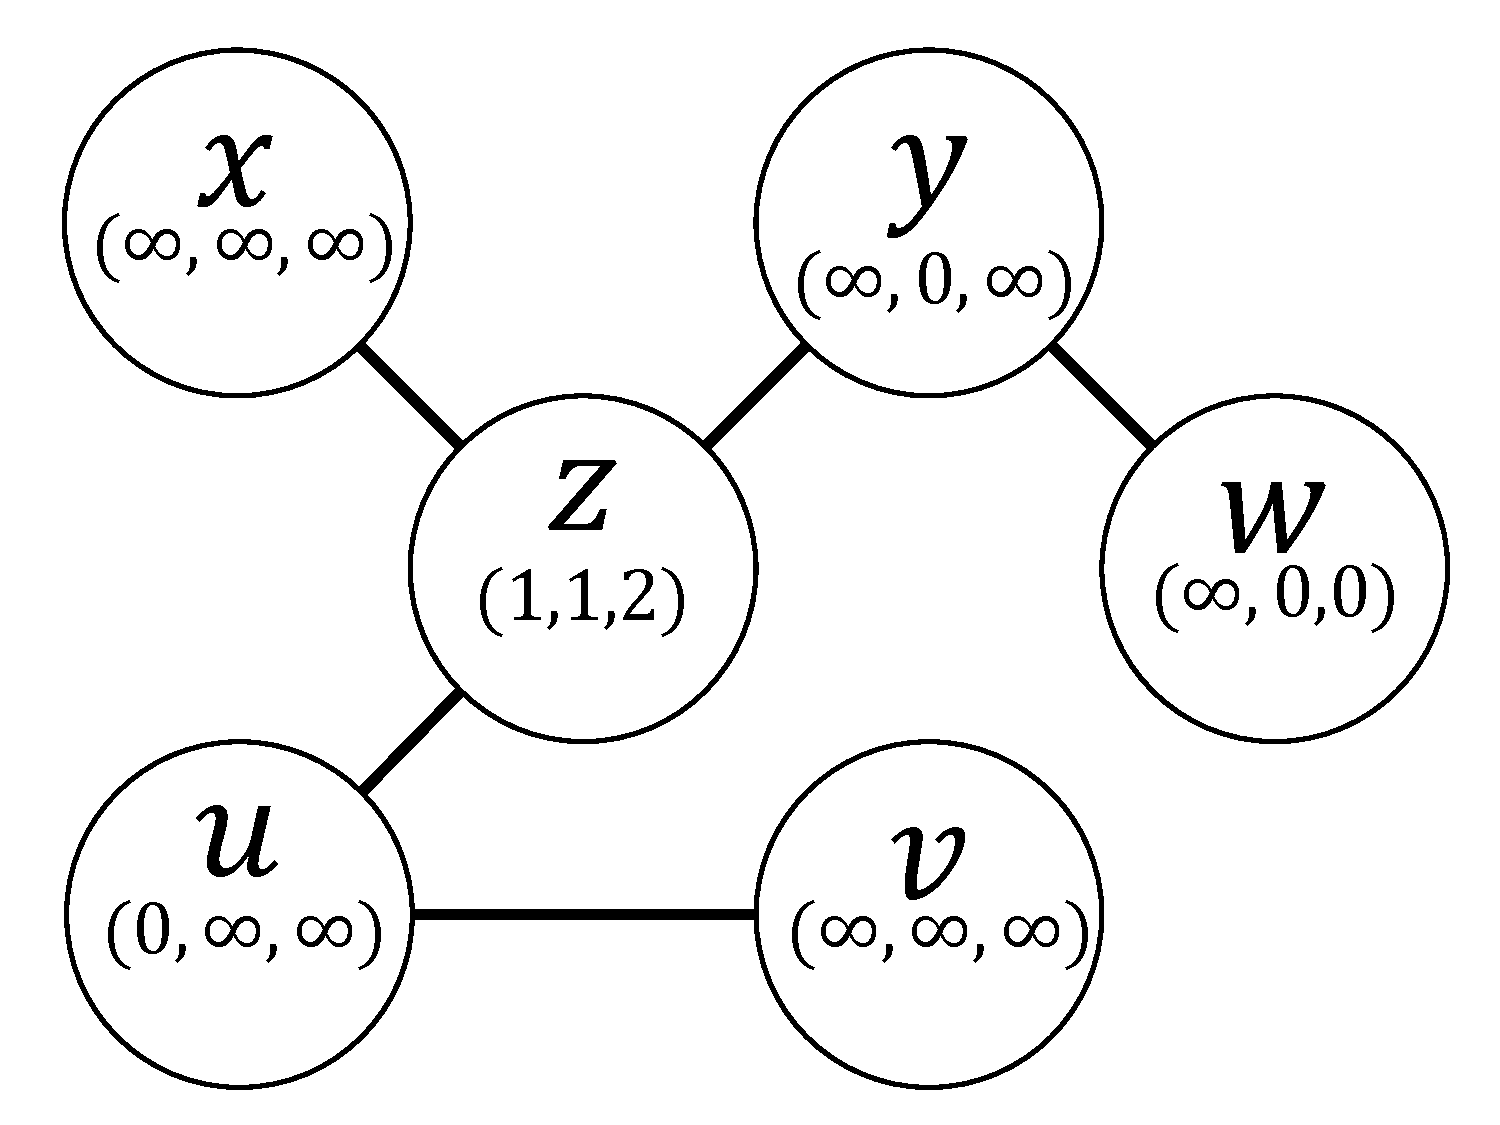
\includegraphics[width=0.5\textwidth]{figs/graph_example_1}
    \caption{\label{font-figure}label distance vector on the first iteration}
    \label{fig:cand_step1}
\end{figure}

\begin{table}[H]
    \centering
    \begin{tabular}{|l|l|l|}
    \hline
      & SDS         & EQS         \\ \hline
    u & A           & $\emptyset$ \\ \hline
    v & $\emptyset$ & $\emptyset$ \\ \hline
    w & BC          & $\emptyset$ \\ \hline
    x & $\emptyset$ & $\emptyset$ \\ \hline
    y & B           & $\emptyset$ \\ \hline
    \end{tabular}
    \caption{\label{font-table}SDS and EQS of each vertex on the first iteration}
    \label{tab:sds_step1}
\end{table}

\begin{table}[H]
    \centering

    \begin{tabular}{|l|l|}
    \hline
    Subspaces & Dominating Candidates \\ \hline
    A         & $(u, dom)$            \\ \hline
    B         & $(w, dom), (y, dom)$            \\ \hline
    C         & $(w, dom)$            \\ \hline
    \end{tabular}
    \caption{\label{font-table}dominating candidates set of each $1$-dimensional subspace on the first iteration}
    \label{tab:cand_set_step1}
\end{table}

Consider the LinkedIn network represented by Table~\ref{tab:skill_sets} and Figure~\ref{fig:graph} as our running example. Again, we take $z$ as the query vertex. The label distance vectors of all vertices are originally initialized as $\infty$. As shown in Figure~\ref{fig:cand_step1}, we start from the vertices with labels and mark the corresponding entries of the label distance vectors of those vertices as $0$. 
We add the label $A$ to $\mathit{SDS}_u$ because $u$ dominates the query vertex $z$ in dimension $A$. Table~\ref{tab:sds_step1} shows the $\mathit{SDS}$ and $\mathit{EQS}$ of all the vertices on the first iteration.
In the first iteration, since $u$ dominates $z$ in the $1$-dimensional subspace $A$, we add $(u, dom)$ to the dominating candidate set $\mathit{CAND}_A$ as shown in Table~\ref{tab:cand_set_step1}.

\begin{figure}[H]
    \centering
    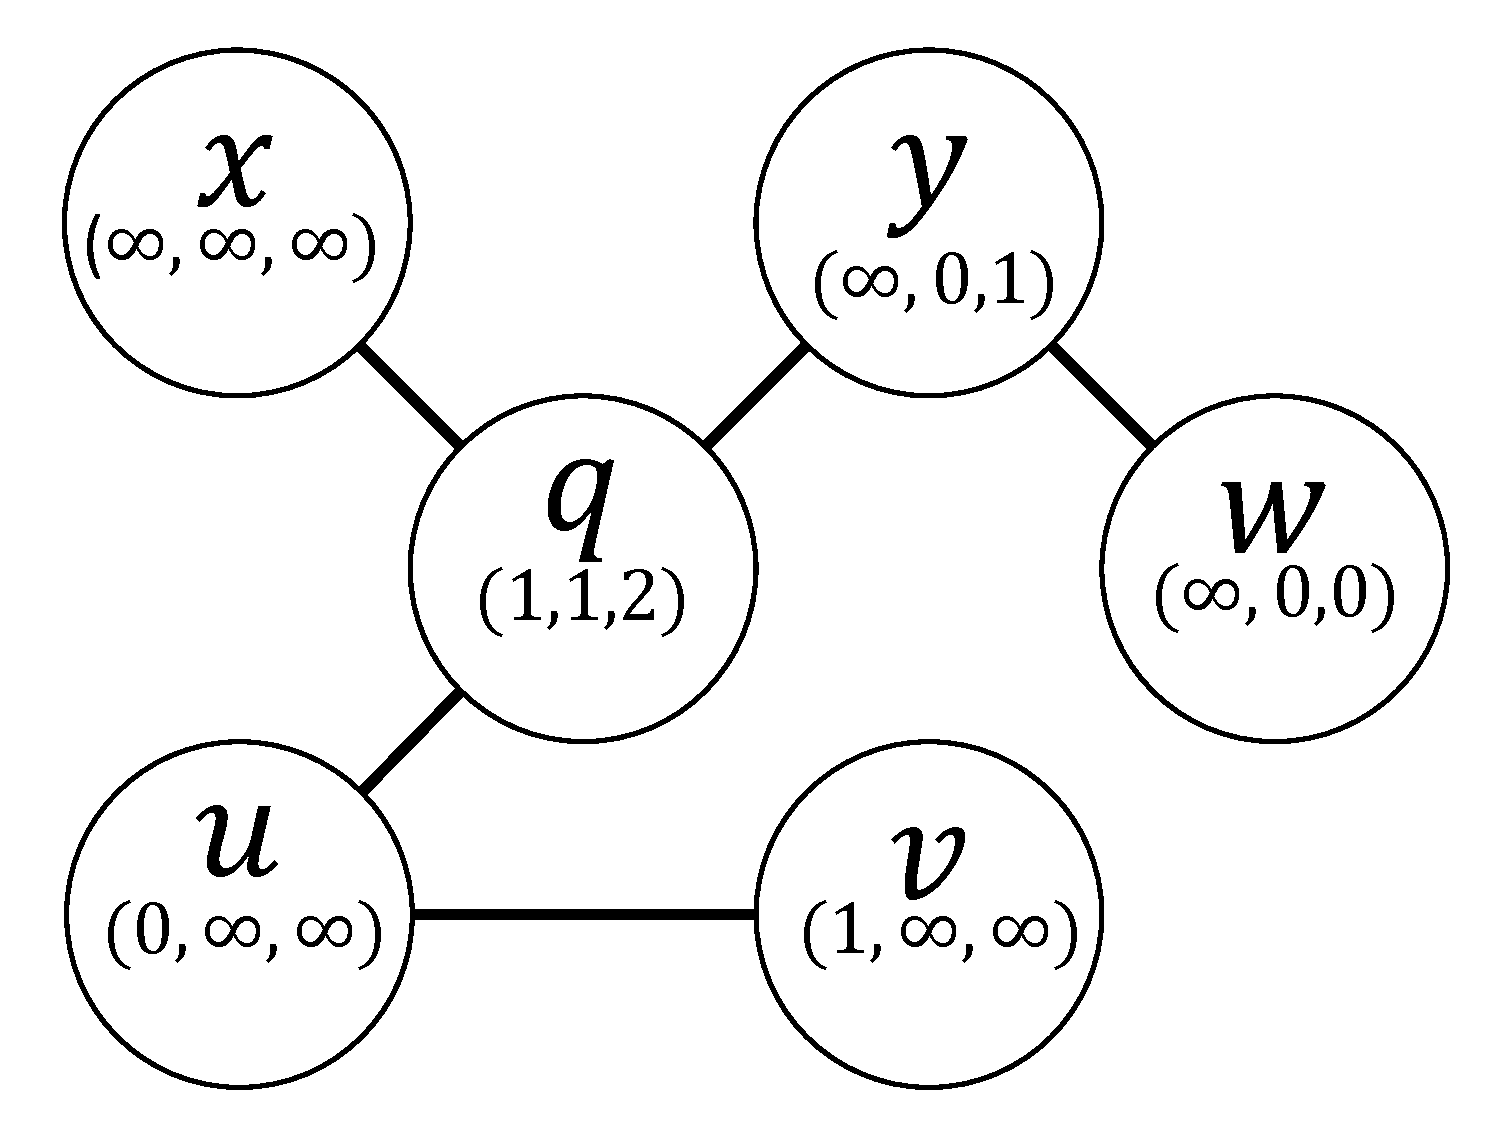
\includegraphics[width=0.5\textwidth]{figs/graph_example_2}
    \caption{\label{font-figure}label distance vector on second iteration}
    \label{fig:cand_step2}
\end{figure}

\begin{table}[H]
    \centering
    \begin{tabular}{|l|l|l|}
    \hline
      & SDS         & EQS         \\ \hline
    u & A           & $\emptyset$ \\ \hline
    v & $\emptyset$ & A           \\ \hline
    w & BC          & $\emptyset$ \\ \hline
    x & $\emptyset$ & $\emptyset$ \\ \hline
    y & BC          & $\emptyset$ \\ \hline
    \end{tabular}
    \caption{\label{font-table}SDS and EQS of each vertex on the second iteration}
    \label{tab:sds_step2}
\end{table}

\begin{table}[H]
    \centering

    \begin{tabular}{|l|l|}
    \hline
    Subspaces & Dominating Candidates \\ \hline
    A         & $(u, dom), (v, eq)$            \\ \hline
    B         & $(w, dom), (y, dom)$            \\ \hline
    C         & $(w, dom), (y, dom)$            \\ \hline
    \end{tabular}
    \caption{\label{font-table}dominating candidates set of each $1$-dimensional subspace on the second iteration}
    \label{tab:cand_set_step2}
\end{table}


Then, we explore the graph in breadth first order. On the second iteration, as shown in Figure~\ref{fig:cand_step2}, we visit the neighbours of the vertices that have been visited on the first iteration and update the corresponding entries of their label distance vectors. Table~\ref{tab:sds_step2} shows that subspace $A$ has been added to $\mathit{EQS}_v$ because on the second iteration we update the distance between $v$ and label $A$ to $2$ which is equal to distance between $z$ and label $A$. For the same reason, we add $(v, eq)$ to $\mathit{CAND}_A$ as shown in Table~\ref{tab:cand_set_step2}. It means that in $1$-dimensional subspace $A$, $v$ is equal to $z$ and it is still possible for $v$ to dominates $z$.

After $2$ iterations, the process of building the  dominating candidate sets of all $1$-dimensional subspace ends. We also finish building the \emph{strictly dominating subspace} and \emph{equivalence subspace} of all the vertices on graph. In figure~\ref{tab:d_hops_distance}, we collect the $3$-hop labels by Breadth-First-Search and get the label vector. By this point, if the value of label $l$ in label distance vertex of vertex $v$ is $\infty$, then it means the distance between label $l$ and vertex $v$ is longer than the distance between the label $l$ and the query vertex $q$.

\begin{table}[h]
    \centering
    \begin{tabular}{llll}
    \hline
    Distances & A & B & C \\ \hline
    $u$       & 0 & $\infty$ & $\infty$ \\ \hline
    $v$       & 1 & $\infty$ & $\infty$ \\ \hline
    $w$       & $\infty$ & 0 & 0 \\ \hline
    $x$       & $\infty$ & $\infty$ & $\infty$ \\ \hline
    $y$       & $\infty$ & 0 & 1 \\ \hline
    $z$       & 1 & 1 & 2 \\ \hline
    \end{tabular}
    \caption{\label{font-table} distances between each person and each skill in 2-hop}
    \label{tab:d_hops_distance}
\end{table}

Although some information is still missing (equal to $\infty$), we are still able to get the mininmal skyline subspaces of $z$: $(A, B)$ and $(A, C)$ from the Table~\ref{tab:d_hops_distance}.

\section{Dominating Candidates Pruning}

In this section, we will introduce a way to prune the unnecessary vertices using the \emph{strictly dominating subspace} $SDS$ and the \emph{equivalence subspace} of the vertices.

\begin{property}
\label{ppt:prune_cand}
Pruning a vertex $u$ from $Cand$ that $\exists v, (SDS_u \cup EQS_u \subseteq SDS_v \cup EQS_v) \wedge (SDS_u \subseteq SDS_v)$, does not affect the result. Therefore, $u$ can be pruned by $v$.
\end{property}

\begin{proof}
Let $v$ be a vertex that $\exists v, (SDS_u \cup EQS_u \subseteq SDS_v \cup EQS_v) \wedge (SDS_u \subseteq SDS_v)$. For any subspace $\mathcal{B}$. Case 1: $q$ is a skyline in subspace $\mathcal{B}$. Then $Cand_\mathcal{B}$ does not contain any elements. Pruning $v$ from $Cand$ does not change the result.
Case 2: $q$ is not a skyline in subspace $\mathcal{B}$ and $q$ is dominated by a vertex $w$, removing $v$ does not change the result. Case 3: $q$ is not a skyline in subspace $\mathcal{B}$ and $q$ is dominated by $u$, then $(\mathcal{B} \subseteq EQS_u \cup SDS_u) \wedge (\mathcal{B} \cap SDS_u \not= \emptyset)$, and there exists such a $v$ that ($SDS_u \cup EQS_u \subseteq SDS_v \cup EQS_v) \wedge (SDS_u \subseteq SDS_v)$. And $(\mathcal{B} \subseteq EQS_v \cup SDS_v) \wedge (\mathcal{B} \cap SDS_v \not= \emptyset)$ is satisfied. Therefore $v$ also dominates $q$ and removing $u$ from $CAND$ does not affect the result.
\end{proof}

One observation is that the unnecessary points is very likely to be pruned by the neighbours of the query vertex $q$. The intuition is that the neighbours of query vertex $q$ will have larger \emph{Strictly Dominating Set} because the query vertex $q$ collects the labels from its neighbours and the neighbours strictly dominate the query vertex in some of the subsets of those labels.
By the Property~\ref{ppt:prune_cand} and the observation above we develop a $1$-hop pruning algorithm. In Algorithm~\ref{algo:pruning_graph}, we compare the $\mathit{SDS}$ and $\mathit{EQS}$ values of neighbours of the query vertex $q$ to all the vertex in the graph in order to prune the some of the candidates in the dominating set.

\begin{algorithm}[H]
  \caption{1-hop Pruning}
  \label{algo:pruning_graph}
  \begin{algorithmic}[1]
  \show\LOOP
    \REQUIRE Strictly Dominating Subspace $\mathit{SDS}$, Equivalence Subspace $\mathit{EQS}$, Dominating Candidates $\mathit{CAND}$, query vertex $q$, graph $G=(V, E)$;
    \ENSURE Pruned Dominating Candidates $\mathit{CAND}$;
    \STATE s = $\left\{v|e(v, q) \in E \wedge (\forall u, e(u, q) \in E \wedge SDS_v \not\subset SDS_u)\right\}$
    
    \FORALL {$(l, dist)$ in $LV_q$}
        \FORALL {$u$ in $\mathit{CAND}_l$}
            \FORALL {$v$ in $s$}
                \IF {$u \not= v \wedge SDS_u \cup EQS_u \subseteq SDS_v \cup EQS_v \wedge SDS_u \subseteq SDS_v$}
                    \STATE delete $u$ from $\mathit{CAND}_l$
                \ENDIF
                
            \ENDFOR
        \ENDFOR
    \ENDFOR
  \end{algorithmic}
\end{algorithm}

\begin{table}[h]
    \centering
    \begin{tabular}{|l|l|l|l|}
    \hline
    Dim & $SDS$       & $EQS$       & $SDS \cup EQS$ \\ \hline
    $u$ & A           & $\emptyset$ & A              \\ \hline
    $v$ & $\emptyset$ & A           & A              \\ \hline
    $w$ & BC          & $\emptyset$ & BC             \\ \hline
    $x$ & $\emptyset$ & $\emptyset$ & $\emptyset$    \\ \hline
    $y$ & BC          & $\emptyset$ & BC             \\ \hline
    \end{tabular}
    \caption{\label{font-table} the $SDS$ and $EQS$ of each vertex}
    \label{tab:SDS_EQS}
\end{table}

Table~\ref{tab:SDS_EQS} shows the $SDS$ and $EQS$ of all vertices on the graph. We can prune the unnecessary vertices from the \emph{dominating candidate set} according this table. By Property~\ref{ppt:prune_cand}, vertex $v$ can be pruned by $v$ and vertex $w$ and $y$ can be pruned by each other.

\begin{table}[h]
    \centering
    \begin{tabular}{lllll}
    \hline
    Distances & A & B & C & Pruned By\\ \hline
    $u$       & 0 & $\infty$ & $\infty$ &\\ \hline
    $v$       & 1 & $\infty$ & $\infty$ & $u$\\ \hline
    $w$       & $\infty$ & 0 & 0 & $y$\\ \hline
    $x$       & $\infty$ & $\infty$ & $\infty$ & $u$\\ \hline
    $y$       & $\infty$ & 0 & 1 & \\ \hline
    $z$       & 1 & 1 & 2 &\\ \hline
    \end{tabular}
    \caption{\label{font-table} label distance vector after 1-hop pruning}
    \label{tab:lv_pruned}
\end{table}

\begin{table}[h]
    \centering
    \begin{tabular}{|l|l|}
    \hline
    Subspaces & Dominating Candidates \\ \hline
    A         & $(u, dom)$            \\ \hline
    B         & $(y, dom)$            \\ \hline
    C         & $(y, dom)$            \\ \hline
    \end{tabular}
    \caption{\label{font-table} Pruned dominating candidate set of $1$-dimensional subspace}
    \label{tab:dom_cand_pruned}
\end{table}

By Table~\ref{tab:lv_pruned}, $v$ and $x$ can be pruned by $u$. Also, $y$ can be pruned by $w$. Table~\ref{tab:lv_pruned} show the vertices to be pruned and their label distance vectors. Although $w$ seems to be a better vertex (because $w$ dominates $y$),  the vertex $w$ is pruned by the vertex $y$ because both vertex $y$ and vertex $w$ have the same \emph{strictly dominating subspace} and \emph{equivalence subspace} and $y$ is a $1$-hop neighbour of the query vertex $q$. Table~\ref{tab:dom_cand_pruned} shows the dominating candidates set of $1$-dimensional subspace after the $1$-hop neighbour pruning.

\subsection{Dominating Candidate Set on Multi-dimensional Subspace}

We generate the dominating candidate set on multi-dimensional subspace by intersecting the smaller dominating candidate set. Since each element in the CAND set of subspace $\mathcal{B}$ has a property \emph{dom} or \emph{eq} representing if that element is dominating query vertex $q$ in subspace $\mathcal{B}$ or equal to the query vertex $q$ in subspace $\mathcal{B}$, we define the CAND set intersection in the following way.

\begin{definition}[CAND Set Intersection]
CAND Set Intersection. $\mathit{CAND}_\mathcal{A} \cap \mathit{CAND}_\mathcal{B} = \left\{(u, OR(x, y)) |\forall u, (u, x)\in \mathit{CAND}_\mathcal{A} \wedge (u, y)\in \mathit{CAND}_\mathcal{B} \right\}$, where $OR(x, y) = equal$ if $x = equal$ and $y = equal$, otherwise, $OR(x, y) = dom$.
\end{definition}

For example, 


\subsection{Subspace Eumeration}
\begin{algorithm}[H]
  \caption{Subspace Eumeration}\label{algo:blah}
    \begin{algorithmic}[1]
  \show\LOOP
    \REQUIRE Dominating Candidates $\mathit{CAND}$ of all one dimension subspaces in $LV_q$;
    \ENSURE A set of subspaces $SUB$ where query vertex $q$ is a skyline;
        \FORALL {$\left(l, dist\right)$ in $LV_q$}
            \STATE if $\exists u, (u, dom)\in \mathit{CAND}_l$, add $l$ to $SUB$, else add $l$ to $L_1$
        \ENDFOR
        \STATE $k$ = 2
        
        \WHILE {$L_{k-1} \not= \emptyset$}
        
            \STATE $C_k = \left\{\mathcal{A} \cup \left\{b\right\} | \mathcal{A} \in L_{k-1} \wedge b \in \bigcup L_{k-1} \wedge b \notin \mathcal{A} \right\}$
            
            \FORALL{(k-1)-subsets $s$ of $c$ do}
                \IF {$s \notin L_{k-1}$}
                    \STATE delete $c$ from $C_k$
                    
                \ENDIF
            \ENDFOR
            
            \FORALL{$\mathcal{C}$ in $C_k$}
                \STATE Let $b$ be the last element in $c$
                \STATE $CAND_\mathcal{C}$ = $CAND_b \cap CAND_{\mathcal{C}-\left\{b\right\}}$
                \STATE if $CAND_l$ is empty, add $l$ to $SUB$, else add $l$ to SUB
            \ENDFOR
            
            \STATE $k$ = $k$ + 1
        \ENDWHILE
        \RETURN SUB
  \end{algorithmic}
\end{algorithm}
